\begin{figure}[ht]
  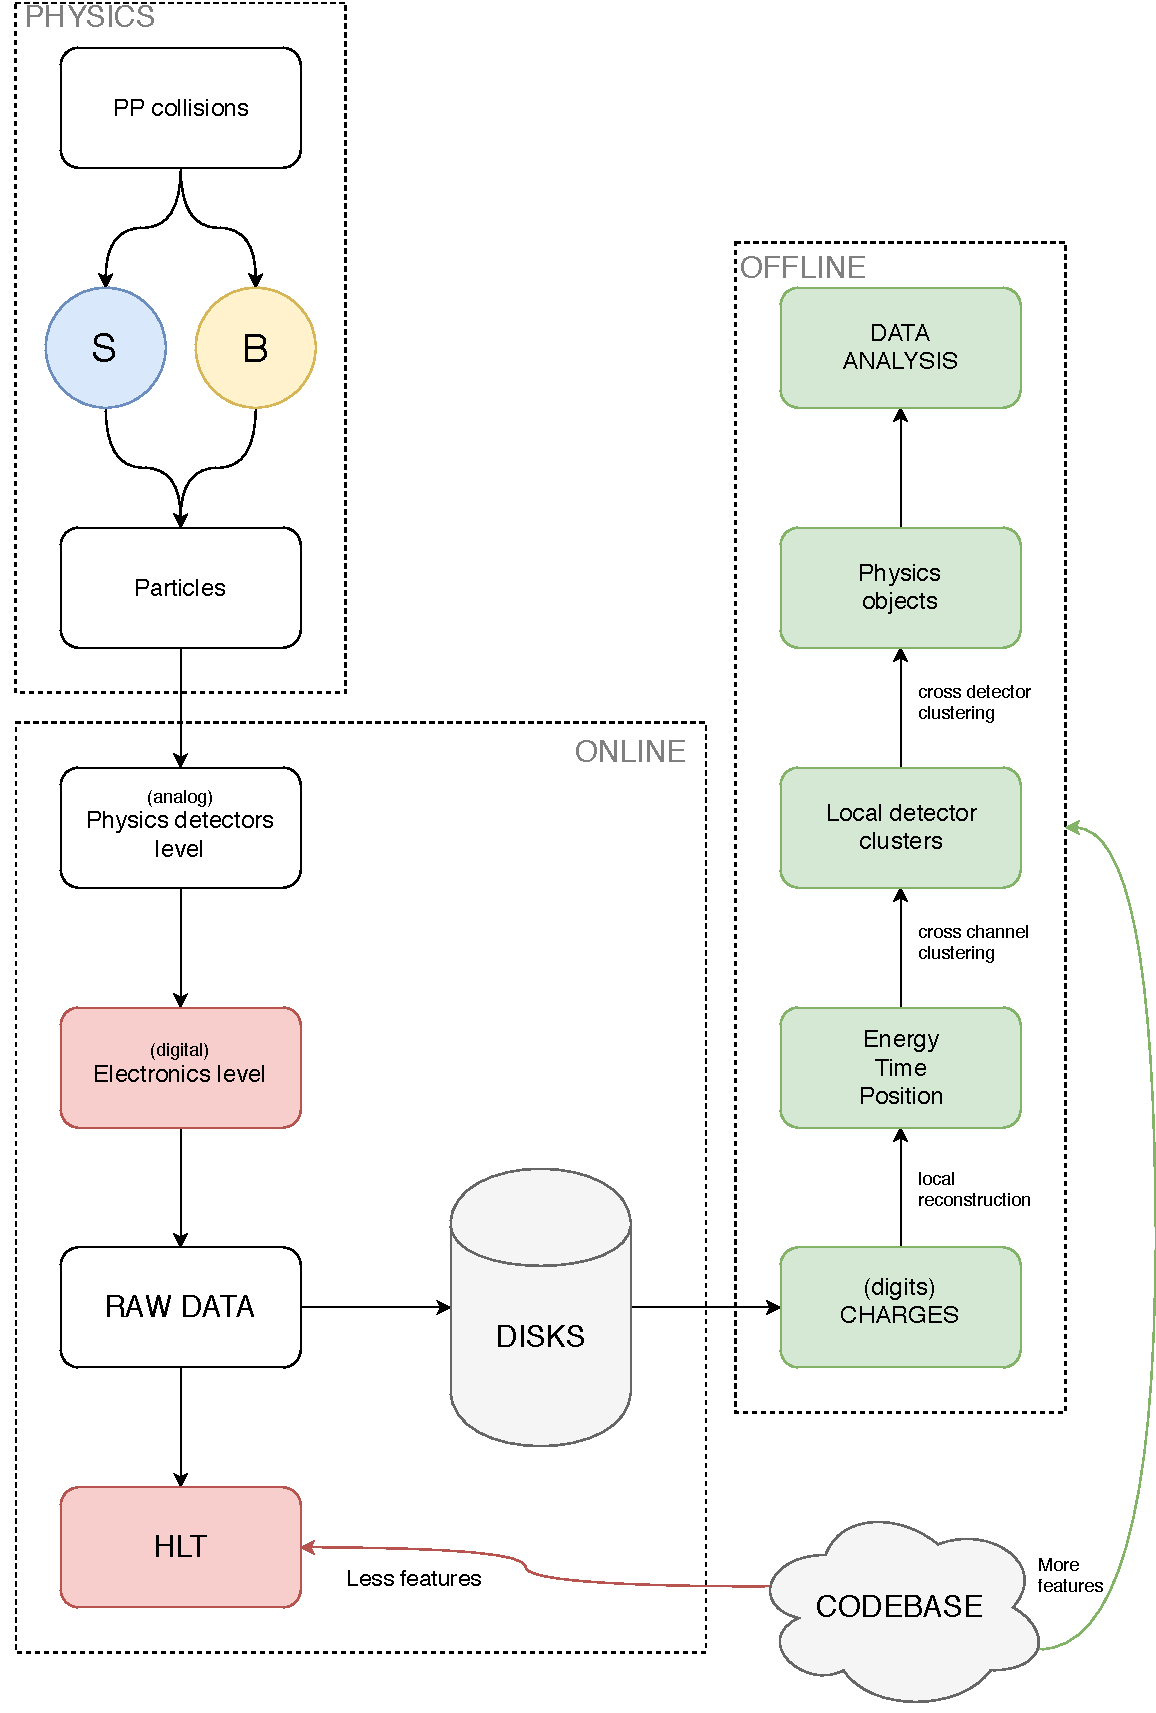
\includegraphics[height=\textheight]{img/dataflow}
  \caption{Cern data flow from collisions to analysis}
  \label{img:dataflow}
\end{figure}

% This might be an introduction\\
Modern \textbf{High Energy Physics} (HEP) experiments require complex multistage infrastructure. To realize them several large scale facilities are needed: from accelerators, detectors, data centers to the thousands of people involved to design and run the infrastructure.\\
%Here at CERN everything starts with physics by colliding particles beams and everything ends with the physics performed by analyzing the data acquired.\\ %But, to produce the necessary data, in the right amount, a long and complicated process, showed in figure \ref{img:dataflow}, is involved. It is worth to briefly describe it to understand the reason of our work and where is it place inside it. \\
The entry point of any \textbf{Large Hadron Collider} (LHC) experiment is the collision between proton-proton beams (although Pb beams are used) which trigger various physical processes. There are two kinds of processes, those that are not yet observed (\textbf{X}) and the observed ones (\textbf{Y}). The objective of LHC experiments is to expand our knowledge about elementary physical processes governing the universe by studying \textbf{X} through the already observed particles that it produces. Unfortunately, interesting processes are quite rare, thus a huge amount of collisions are needed to produce one of them.\\
This creates a lot of difficult and interesting IT challenges because everything from data acquisition to data analysis has to scale to meet throughput and timing requirements. The faster data are processed, more collisions can be triggered therefore, quicker the research can proceed.\\
As computer scientists, our purpose here at CERN is to accelerate data processing by best exploiting the resources at our disposal, achieving the maximum efficiency using smart and creative approaches, in particular targeting \textbf{High Performance Computing} (HPC) environment. \\
The LHC infrastructure is designed to process huge amounts of data (hundreds of Pb/s). The data flow architecture illustrated in figure \ref{img:dataflow} is organized in four main stages. Staring from physical processes to the physics carried out by analyzing the data, with data acquisition and processing in the middle. Each of this step is complex and deserves a dedicated explanation. 
\paragraph{Data generation}
The process starts with beams of \textbf{protons} colliding every $25ns$ that leads to particle interactions that create some \textbf{intermediate products}. These intermediate products can not be directly observed, but they further decay into something observable by the detectors.
\paragraph{Data aquisition}
Detectors are split in two levels: \textbf{physics detector level} and \textbf{electronics level}. The physics level takes in input sensor readouts and produces an analog signal. This analog signal is digitalized by the electronics level. At this point there is too much data to send it directly to the next stage. Models are used to distinguish between which data that belongs to X and which one belongs to Y. Since these models are complex and the timing constraints are very strict, only a simplified version of them is implemented directly in hardware, on top of \textbf{Application Specific Integrated Circuit}s (ASIC) and \textbf{Field Programmable Gate Array}s (FPGA) boards. Because the models are simplified there are a lot of Y events labeled as X. \\
% Should I say that not interesting reading are discarded here?
The events that survive this first stage are sent to the \textbf{High Level Trigger} (HLT).\\
The HLT has more relaxed time constraints since it receive less events and its job is to distinguish between X and Y exploiting, an implementation of the same models used inside the previous stage, but with more features that allows more precise evaluations. Another important characteristic of the HLT is that is implemented in software and executed on a CPU based cluster. Currently there is an attempt to integrate and exploit accelerators such as GPUs and FPGAs inside this cluster.
\paragraph{Data processing} 
At this point, events that pass previously described two level trigger system are used to generate a dataset used for analytics purposes. To build this dataset the same models deployed inside the triggers are used, but with way more features. To extrapolate useful information and build the dataset \textbf{raw data} are sent through a complex multistage processing pipeline. This pipeline is offline so it does not share the timing constraints of the previous stage but, efficient exploitation of resources is needed because even after all the filtering data is still huge and models are very complex. \\
The first stage, called \textbf{local reconstruction}, transforms charges to physical quantities such as \textbf{energy}, \textbf{time}, and \textbf{position}. This operation is done channel by channel. These channels are independent form each other thus, this is an embarrassingly parallel problem. This parallelism is exploited though multi-threading running this code on a cluster of multi-core machines, although other parallel architectures, such as GPUs, are currently tested to deploy them in future upgrades. Then, information coming from different channels of the same detector are combined by the \textbf{cross channel clustering} into \textbf{local detector cluster}s. The final step needed to obtain \textbf{particle object}s is the \textbf{cross detector clustering} in which data coming from different detector is combined. In the end, some particle objects are built. The set of all these particle objects form the dataset used to probe new horizons of fundamental physics.\\
% \paragraph{High level trigger (HLT)}
% The \textbf{HLT} belongs both to data acquisition and data processing, since it would not be correct to include it in one of this categories, it deserves a separate discussion. \\
% The HLT main purpose is to select interesting events before writing them to disk. In order to accomplish this, it runs the same code used for the offline processing, but \textbf{online} and with less features because of strict time constraints. \\
% The main difference between \textbf{L1} and HLT is that L1 is implemented in hardware with no host while HLT is software based, it runs on hosts with accelerators used to speed-up the processing.
